% This Latex template file set ups a two column paper with several
% options. 
% The ACM option (to be set inside preamble.sty)
% The Usenix option (to be set inside preamble.sty)
% It also implements (as options) space saving and commenting options
% (also in preamble.sty)

% When using Usenix, choose this: 
% \documentclass[letterpaper,twocolumn,10pt]{article}
% When using ACM, choose this
\documentclass[sigplan,review]{acmart}
\renewcommand\footnotetextcopyrightpermission[1]{}
\settopmatter{printfolios=true,printacmref=false}

\usepackage{preamble}

\begin{document}
\title{Bigger, not Badder: Safety of Scaling Byzantine Protocols}

\author{David C. Y. Chu}
\orcid{0000-0001-9922-1994}
\affiliation{
    \institution{University of California, Berkeley}
    \country{USA}
}
\email{thedavidchu@berkeley.edu}

\author{Chris Liu}
\orcid{0009-0002-1880-1941}
\affiliation{
    \institution{University of California, Berkeley}
    \country{USA}
}
\email{chris-liu@berkeley.edu}

\author{Natacha Crooks}
\orcid{0000-0002-3567-801X}
\affiliation{
    \institution{University of California, Berkeley}
    \country{USA}
}
\email{ncrooks@berkeley.edu}

\author{Joseph M. Hellerstein}
\orcid{0000-0002-7712-4306}
\affiliation{
    \institution{University of California, Berkeley}
    \country{USA}
}
\email{hellerstein@berkeley.edu}

\author{Heidi Howard}
\orcid{0000-0001-5256-7664}
\affiliation{
    \institution{Azure Research, Microsoft}
    \country{UK}
}
\email{heidi.howard@microsoft.com}

\begin{abstract}
Distributed protocols such as 2PC and Paxos lie at the core of many systems in the cloud, but standard implementations do not scale.
New scalable distributed protocols are developed through careful analysis and rewrites, but this process is ad hoc and error-prone.
This paper presents an approach for scaling \emph{any} distributed protocol by applying rule-driven rewrites, borrowing from query optimization.
Distributed protocol rewrites entail a new burden: reasoning about spatiotemporal correctness.
We leverage order-insensitivity and data dependency analysis to systematically identify correct coordination-free scaling opportunities.
We apply this analysis to create preconditions and mechanisms for coordination-free decoupling and partitioning, two fundamental vertical and horizontal scaling techniques.
Manual rule-driven applications of decoupling and partitioning improve the throughput of 2PC by $5\times$ and Paxos by $3\times$, and match state-of-the-art throughput in recent work.
These results point the way toward automated 
optimizers for distributed protocols based on 
correct-by-construction rewrite rules.
\end{abstract}
\maketitle


\section{Introduction}
\label{sec:intro}
\david{BFT is popular but throughput is difficult to scale.}
Dealing with arbitrary failures is inherently complex; dealing \emph{efficiently} with arbitrary failures even more so. 
Designing correct, scalable BFT~\cite{byzantineGenerals} protocols is thus extremely challenging, and even experts often make mistakes~\cite{zyzzyvaBug, protocolBugsList}.
While one cannot do much about the inherent complexity of BFT, recent work suggests an appealing middle ground.
Instead of creating new, scalable protocols from scratch, one can break down existing (and usually simpler)
% \natacha{and usually simpler?}
protocols into components~\cite{chemistryBehindAgreement} that can be scaled individually~\cite{compartmentalized}.

Gupta et al.~\cite{resilientdb} manually pipelined and partitioned existing BFT protocols, achieving up to $6\times$ throughput improvement.
\sigmodpaper{}~\cite{autocomp,autocompTechReport} obtained similar results with simple, local, \emph{program rewrites} for Paxos~\cite{paxosComplex}: \textbf{decoupling} (splitting logic across nodes) and \textbf{partitioning} (splitting data across nodes), as seen in \Cref{fig:rewrites}.
Their rewrites are promising because they are protocol-agnostic and rule-driven: given a protocol written in a distributed DSL~\cite{dedalus}, the rewrites can be used to correctly modify any protocol.
However, these rewrites were proven correct assuming non-Byzantine failures only.

This paper modifies the rewrites introduced by \sigmodpaper{} and proves the correctness of the resulting rewrites when applied to BFT protocols.
% In this paper we investigate the vulnerability of these rewrites to Byzantine attacks, and we enhance the rewrites to provably tolerate Byzantine behavior.
% \jmh{Rather than end on a negative note, end on a plan: "HOwever, these rewrites were proven correct assuming non-Byzantine failures; this weakness makes the rewrites unsafe for optimizing BFT protocols. In this paper we investigate the vulnerability of these rewrites to Byzantine attacks, and we enhance the rewrites to provably tolerate Byzantine behavior. [Paragraph Break] To illustrate the vulnerabilities of the rewrites in Chu et al., consider..." Then you can delete the short paragraph after this one.}
% \david{Joe: State that it would be good to apply them to BFT. Emphasize that it's our hypothesis. Natacha: Cite Suyash's work on ResilientDB breaking down protocols into components}
% \natacha{Maybe Suyash's work fits better here. I would love to see a sentence here that talks about the potential win. "This is a missed opportunity. Gupta et al. shows that with careful engineering, pipelining, etc. BFT protocols can be made up to Xxx faster without any algorithmic changes}

% \david{Provide example of unintuitive new vector of attack: partitioning}
% To illustrate the challenge, consider a simple vote-counting protocol that stores votes in a set.
% It exposes two APIs: \texttt{appendVote(id)} and \texttt{count()}.
% The \texttt{appendVote(id)} function verifies each vote before inserting it into the set.
% The \texttt{count()} function hash partitions votes by id, counts the number of votes in each partition, then sums up the counts across partitions.
% Because votes with different ids are independent, \sigmodpaper{}'s rewrites assert that this set as a whole can be partitioned and distributed across nodes.

% Let us assume that this set is BFT, but Byzantine nodes can interact with it via API calls.
% In the presence of Byzantine failures, partitioning would be \emph{unsafe}.
% A Byzantine node could send the same, valid, vote to multiple nodes, inflating the final count.
% Because the partitioning rewrite was not designed to handle Byzantine failures, individual nodes do not verify whether the partitioning invariant is violated \nc{They do, just not the same invariant as in the CFT?} and become vulnerable to duplication attacks.
% In general, without modifications, the rewrites presented by \sigmodpaper{} are unsafe when applied to BFT protocols.
% \david{Natacha: Make clear that we need to modify the partitioning rewrites, not the invariants. Make clear what would have happened before partitioning (votes cannot be inserted multiple times). Think about BFT example where this would be a problem where the original protocol was completely BFT? Would be nice if example was PBFT. Example: decoupling, 1 original node sending its prePrepare to the committer. Can send different command; the committer doesn't re-check that the digest matches the command.
% Joe: Another possibility: don't give full self-contained example. Just say what could go wrong with decoupling and partitioning.}

\begin{figure}[t]
    \centering
    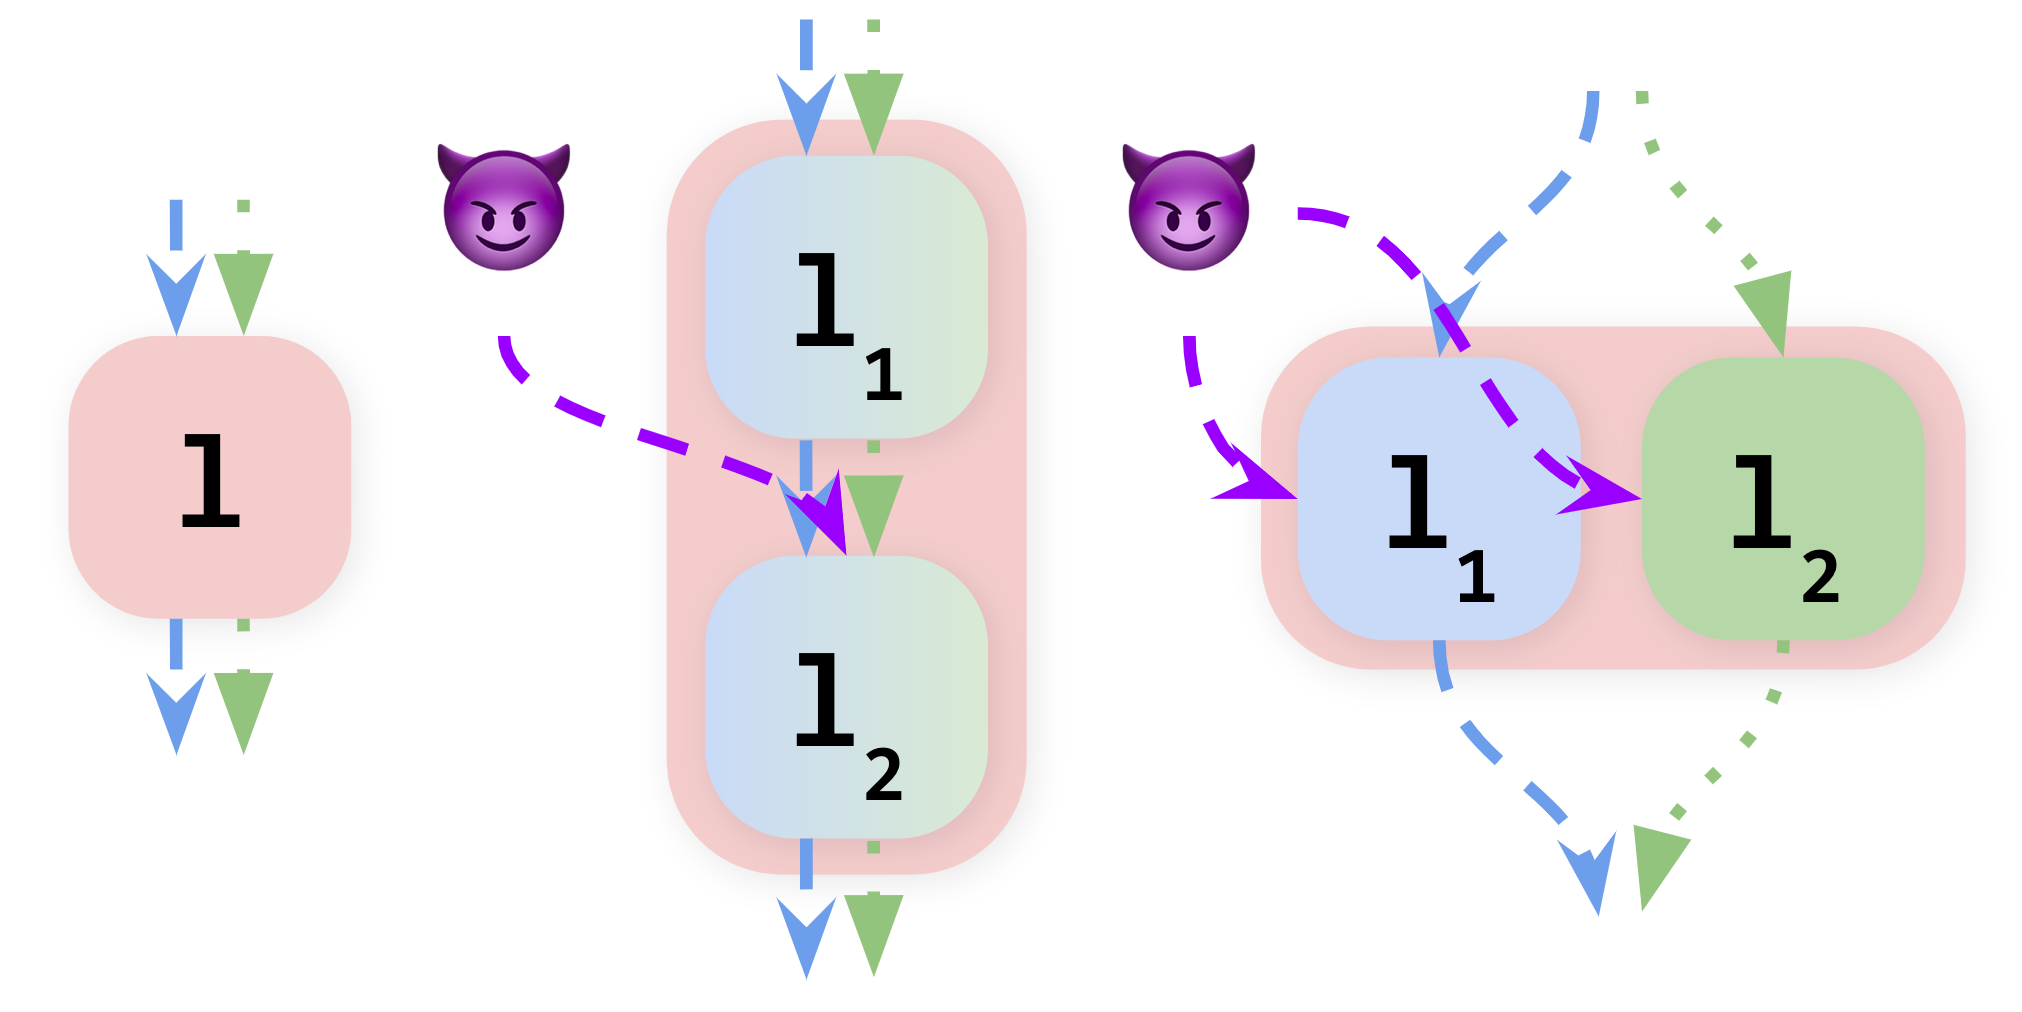
\includegraphics[width=0.8\linewidth]{assets/rewrites.png}
    \caption{Decoupling (middle) and partitioning (right), splitting a node $l$ into two nodes $l_1$ and $l_2$. Byzantine nodes (evil emoji) can insert messages on decoupled message channels and duplicate messages across partitions.}
    \label{fig:rewrites}
\end{figure}


\david{Example of vector of attack: decoupling on PBFT.}
To illustrate the challenge, consider the critical path of PBFT~\cite{pbft}, a fundamental BFT protocol that reaches consensus across $3f+1$ replicas.
Replicas in PBFT receive \textsc{PrePrepare} messages from a primary replica: these messages contain, among other things, a command to execute, its hash digest, and a signature from the primary over the hash digest.
The replica accepts the message if the digest is indeed the hash of the command and the signature is valid.
In a later phase, once this replica receives $2f+1$ \textsc{Commit} messages (which also contain a digest) from other replicas, it will compare the digest within the \textsc{Commit}s to the digest of the \textsc{PrePrepare} it received earlier; if the digests match, then the replica will execute the command.

Because the replica monotonically accumulates sets of \textsc{PrePrepare} and \textsc{Commit} messages through time, the rewrites from \sigmodpaper{} suggest that replicas can be scaled up via monotonic decoupling.
% \tyler{For a single node,} 
For each node, the logic that collects \textsc{PrePrepare} messages and the logic that collects \textsc{Commit} messages can be decoupled into two nodes: a \emph{pre-preparer} and \emph{committer} \jmh{reference Figure 1 here to illustrate. I recommend you change it to Fig 1a and 1b, one each for decoupling and partitioning, so that here you can reference "$l_1$ and $l_2$ of Figure 1a", rather than "$l_1$ and $l_2$ of the middle of Figure 1"?}.
% \tyler{two nodes, a pre-prepreparer and committer, where the pre-preparer forwards \textsc{PrePrepares} to its own committer, which later compares digests and executes the command.} 
Crucially, each pre-preparer \jmh{(e.g. $l_1$)} must forward \textsc{PrePrepare}s to its own committer \jmh{($l_2$)}so it can later compare digests and execute the command.
The remaining phases of PBFT can be similarly decoupled, as we will discuss in detail in \Cref{sec:eval}.

% \tyler{Intuitively, decoupling logic into two nodes increases the parallelism and therefore the throughput of the system. However,}
Intuitively, decoupling logic into two nodes reduces load on any one machine and can improve throughput.
However, in the presence of Byzantine failures, this decoupling would be \emph{unsafe}.
A single Byzantine node could \jmh{masquerade as two pre-preparers, and} send two committers doctored \textsc{PrePrepare}s with the same digest but different commands.
Committers, without checking whether the message was forwarded from their own pre-preparers, would then execute the wrong commands, breaking the consensus invariant.
Because \sigmodpaper{}'s decoupling rewrite was not designed to handle Byzantine attacks, the messages between decoupled nodes are neither signed nor verified, allowing Byzantine nodes to insert their own messages as seen in \Cref{fig:rewrites}.


% \natacha{What is the flow you were going for for the next 3/4 paragraphs? It's hard to follow the order. }
% \natacha{Is it the rewrites that are different, the conditions on which you can apply them, or just the proofs? You switch between all of them and it's a bit confusing.}
% \natacha{I'd shorten the next paragraph to be more direct. We first address two challenges, etc. First, we must precisely model all possible Byz behaviour in the system. If the non-scaled protocol is correct in a world in which all Byz behaviour is possible, the scaled protocol should also be correct. Byz nodes can execute arbitrary program logic and send arbitrary messages .. }

% \david{Why rewrites are vulnerable and how we modify them.}
% \natacha{Would be nicer to talk in terms of challenges and solutions? What are he two/three challenges you had to address, and then describe how your solution addresses those. I would say there are two challenges 1) how to actually model correctness (for this you need to express all possible Byz behaviour}
% We modify the rewrites by hardening message channels introduced by decoupling and partitioning against Byzantine attacks.
% Decoupling converts dataflow within a single-node process into message channels between nodes, which Byzantine nodes can populate with arbitrary messages. We modify decoupling such that messages on these channels are signed and verified.
% \natacha{Why do you need signatures rather than MACs?}\heidi{Transferability?}
% Partitioning splits messages across nodes; Byzantine nodes can send messages to incorrect partitions.
% We modify partitioning such that nodes check whether the message they receive belongs to their partition.
% \david{How we prove correctness.}
% In order to prove the correctness of our modified rewrites, we will demonstrate the following:
% (1) Byzantine nodes can be modeled \jmh{by a "randomization construction" or some such name} \emph{entirely based on the output they produce},
% (2) Byzantine nodes in a protocol that has been rewritten are no more powerful than Byzantine nodes in the original protocol, and
% (3) Message channels introduced or modified by the rewrites are safe against Byzantine nodes.

% \david{Heidi: Introduce rewrites.}
\david{Our rewrites.}
To prevent the attack above, we will modify decoupling with \emph{sender verification} (\Cref{sec:sender-verification}), which signs and verifies each message sent between decoupled nodes.
We will also modify partitioning with \emph{message verification} (\Cref{sec:message-verification}), such that each partition individually verifies that it is receiving the correct subset of hash-partitioned messages.

\david{Our proof strategy.}
% \jmh{Given an input protocol that is BFT...?}
Given an input protocol that is BFT, our proof strategy is two-fold: we show that (1) to nodes untouched by the rewrites, Byzantine nodes in the rewritten protocol cannot generate any more messages than they could have generated before, and
\david{Natacha: Change all instances of ``compare Byzantine behavior'' or power to discussion on how Byzantine nodes can't send more things that they could have sent before.}
(2) for modified nodes, all invariants required by the rewrites are reinforced against Byzantine attacks.
With these guarantees, any Byzantine attacks on the untouched nodes in the rewritten protocol would be identical to a Byzantine attack in original protocol (which is already BFT), and any Byzantine attacks on the modified nodes are ineffective.

\david{Modeling Byzantine behavior.}
In order to discuss what messages a Byzantine node can produce, we must formally model \emph{all} possible Byzantine behavior as part of our proof framework.
This is tricky: Byzantine behavior is, by definition, arbitrary.
% , with the caveat that one cannot break standard cryptographic primitives.
To this effect, we make the following observations: (1) a Byzantine node's behavior is a function of its outputs, and (2) the set of all possible Byzantine behaviors is 
% \jmh{eventually executed by nodes that execute random behaviors?} 
exactly the set of all \emph{random} behaviors.
% \tyler{Do you need to emphasize randomness to prove correctness? My worry is that randomness might suggest to a reader that you might empirically evaluate your correctness with e.g. fuzzing as opposed to a formal proof. The proof-of-correctness in section 5 does not seem to require randomness at least to my understanding.}
We introduce the \emph{\randomSimulator{}}\footnote{Jorge Luis Borges' story \textit{The Library of Babel} posits a library of books composed of every possible ordering of characters. By definition, this library contains all books, though it may take arbitrary time to find good ones.}, a theoretical gadget that simulates all possible Byzantine behavior in a protocol-agnostic way through randomness.
At any point in time, the \randomSimulator{} can generate arbitrarily many random messages to all input channels.
This theoretical gadget allows us to compare Byzantine behaviors and prove the correctness of the modified rewrites.

% \natacha{The bullet structure is a bit strange -> (3) is the end goal and (2)/(1) are necessary steps to achieve 3. Putting them as the same "level" is confusing. I would rephrase as follows: }
% \natacha{The key challenge in proving correctness in a BFT setting stems from having to model *all* possible Byzantine behavior as part of our proof framework, before showing that the set of behaviour post rewrites is a strict subset of allowable behaviour in the original protocol. Byzantine behaviour is, by definition, arbitrary. Nodes cannot break standard cryptographic primitives but can otherwise behave in arbitrary ways.  To this effect, we introduce the Borgesian simulator, a gadget that simulates all possible Byzantine behaviour in an protocol agnostic way by allowing Byzantine nodes to behave randomly. At any given point in time, the Borgesian gadget can generate infinitely many random messages to all input channels}


% The power of \randomSimulator{}s can be compared on the cryptographic keys they have access to, the signed messages they have received, and the input channels they can send to. \natacha{I can't understand this sentence}
% We will show that our rewrites do not allow Byzantine nodes access to more keys \natacha{What does it means for nodes tohave additional keys?} additional messages that they can receive are useless, and that the new and modified input channels are resilient against Byzantine messages. \jmh{This last sentence is not apropos to the topic sentence of the paragraph. Maybe doesn't belong in this paragraph?}

\david{Results.}
Our initial results are promising.
The modified rewrites are simple to check, yet applying them scales the throughput of PBFT by $5\times$ when applied to its critical path.
% \david{Should we end this paragraph with some implications of the larger picture?}

% The difference in the proofs used by this paper and \sigmodpaper{} can be boiled down to the difference in what messages a correct machine can receive.
% \sigmodpaper{} made two implicit assumptions in their rewrites that do not hold in a Byzantine environment:
% (1) New machines will execute program logic as intended, and
% (2) Modified input channels will be populated with the expected messages.

% The first assumption is violated if a new machine becomes Byzantine. \heidi{there was a switch here from nodes to machines, i prefer nodes}
% We will show that new Byzantine machines are no more powerful than Byzantine machines in the original protocol.
% \chris{"...no more powerful than old Byzantine machines that existed before protocol rewrites"?}
% In order to prove this property, we must carefully define what messages Byzantine machines are capable of sending.

% The second assumption is violated if Byzantine machines attempt to violate the modified input channels' invariants, as in the partitioning example presented earlier. \nc{Not sure I get that}
% \jmh{Note that in the set-of-votes example above, the invariant is explicit: to ensure local duplicate detection works, input channel must obey partitioning.}
% We will modify the rewrites such that nodes detect and discard any invariant-violating messages.
\section{Background}
\label{sec:background}
\textbf{Rule-driven rewrites.}
\sigmodpaper{} presents a set of rule-driven rewrites that can be applied to arbitrary distributed protocols if the preconditions are met.
Rewrites improve protocol throughput by scaling up, spreading the logic or data of an individual machine $m$ across multiple machines $m_1, m_2, \ldots$ through decoupling and partitioning, respectively.
When a machine $m$ is scaled up in this way, new input channels may be introduced between its new machines $m_i$ in order to transfer data, and machines that previously sent messages to $m$ may need to forward messages to a specific machine in $m_i$ or duplicate the message to all machines $\overline{m_i}$.

\sigmodpaper{} proved the correctness of the rewrites over Dedalus~\cite{dedalus}, a declarative dataflow language for distributed systems based on Datalog.
Due to limited space, we will instead discuss rewrites over event-driven pseudocode instead.

\textbf{BFT.}
BFT protocols can tolerate up to $f$ Byzantine failures, where Byzantine machines can send arbitrary messages and share private keys, although they cannot break cryptography~\cite{pbft}.
We assume a shared-nothing architecture in which machines can only communicate through messages, and messages between correct machines will eventually be delivered.
Note that this paper is focused on proving the correctness of \emph{rewrites} across BFT protocols, not the correctness of any specific BFT protocol.
We will use PBFT~\cite{pbft}, a foundational BFT protocol, as a case study in our proofs.

\textbf{Correctness.}
Correctness is defined by the observable program behavior.
A rewrite is correct if given any program $P$, a rewritten program $P'$, and any set of inputs (and their respective send times), $P'$ always generates the same outputs with the same timestamps as some possible run of $P$~\cite{autocomp}.

% Note that the fault tolerance of a protocol does not change as a result of scaling up.
% The Byzantine failure of any new machine $m_i$ is equivalent to the failure of the original machine $m$. \chris{This part may need more elaboration since it might not be immediately obvious to new readers, or we should at least mention again that we will prove this later}

\section{\randomSimulator{}s}
\label{sec:bft-formalism}
To prove the correctness of rewrites in a Byzantine setting, we must first formally model a Byzantine node in a protocol-agnostic way.

\david{Only the messages BFT nodes send are relevant.}
This is tricky; a Byzantine node can execute arbitrary logic.
Fortunately, other nodes only observe the output of the node, not the logic by which it generated a particular message.
Two Byzantine nodes that generate the same outputs are indistinguishable, even if one executes complex logic and the other creates messages at random.
% A Byzantine node that executes complex logic in order to produce message $m$---and a Byzantine node that just happens to produce message $m$ by luck---are indistinguishable.
It follows that a Byzantine node can be modeled solely by its outputs.
% As Byzantine nodes can execute arbitrary logic, they can generate arbitrary messages, and arbitrarily many of them.

Byzantine behavior can thus be fully captured by a \emph{random message generator}: if, at each point in time, a node sends a random number of random messages to each channel, then that node must contain, in its set of possible runs, \emph{exactly all} possible runs of any Byzantine node.
We name this random message generator the \textbf{\randomSimulator{}}.
This simulator can generate both nonsensical and seemingly intelligent outputs, all of which must be correctly handled by a BFT protocol.
% Although BFT protocols often prove correctness against a malicious adversary, they must be safe against arbitrary attacks; indeed, recent work suggests that correct nodes with random state and message permutations can appear Byzantine and help expose bugs in BFT protocol implementations~\cite{twins}. \natacha{Don't understand the last sentence, what are you trying to say?}
We will formalize the \randomSimulator{} by attaching a \textbf{\randomHarness{}} to all nodes in a BFT protocol.
Note that this harness defines what a protocol must defend against 
% \jmh{rather than ``allows us to simulate'' how about ``requires a protocol to defend against''} 
and is \emph{not} meant to be applied in practice or used as a fuzz tester.

% A formal specification of the expressivity of Byzantine machines is necessary in order to prove the correctness of rewrites in a Byzantine setting.
% \natacha{I'm not a big fan of the phrasing "specification of expressivity". We we say instead: W To prove the correctness of rewrites in a Byz setting, we must first formally model the fact that Byz nodes can deviate from the protocol arbirarily, send arbitrary messages (1), without breaking cryptographic primitives (2). We address each in turn.}
% \natacha{Might be helpful to remind the reader of what Byz nodes can and can't do in general, and then you talk about how you go about modeling this in your work}
% We can reduce a Byzantine machine down to the messages that it sends (and does not send).
% Their internal state is 
% % largely \heidi{remove largely} 
% irrelevant, aside from their ability to reuse messages that they have previously received, which we will discuss in \Cref{sec:signed-channels-formalism}.\natacha{This is a neat idea. Could you make a bigger deal out of it maybe? Byz nodes can deviate arbitrarily from the protocol -> wow this seems hard -> in practice, we can actually ignore tha tpart and just look at the messages that they send since that's the only "external" impact that they have on the ssytem and that's what trace equivalence is based on}

% We will encode a Byzantine machine's ability to send arbitrary messages as theoretical rewrites that append logic to each machine \natacha{Could not parse that sentence at all, sorry}.
% These pieces of logic are conditioned on the boolean \texttt{isByzantine(l)}, where \texttt{l} is the machine's location identifier, and \texttt{isByzantine(l)} is true for at most $f$ unique locations.
% Byzantine machines not only have the ability to send arbitrary messages, they can also ignore their assigned roles and refuse to execute existing logic: we formalize this flexibility by conditioning all existing logic on \texttt{!isByzantine(l)} 
% \natacha{I'm not entirely sure that others will be able to follow what you're saying here. I can because I know what you do, but I'm not sure others will. "pieces of logic", "conditioned on" is quite vague. It'd be a lot easier I think with an example (see above)}.

% \david{Not breaking cryptography.}
% Most \natacha{All?} BFT protocols also assume that Byzantine machines cannot break cryptography~\cite{pbft}.
% Therefore, we must distinguish between message fields for which a Byzantine machine can send arbitrary data, and fields that encode cryptographic information.
% \natacha{Do we want to be more precise here? It's not the case that they can't send arbitrary data and then encrypt it themselves, it's that they can't spoof the credential of other replicas?}
% We assume that each message channel is strongly typed and annotated with their cryptographic guarantees \natacha{What does it mean for a channel to have cryptographic guarantees?}.

% We will formalize what messages a Byzantine machine can send based on the message types used in PBFT~\cite{pbft}: plaintext messages (\Cref{sec:plaintext-channels-formalism}), signed messages (\Cref{sec:signed-channels-formalism}), and certificates and nested types (\Cref{sec:certificate-channels-formalism}). \natacha{What is the difference between a signed message and a certificate, and what is a nested type?}

\subsection{Plaintext message channels}
\label{sec:plaintext-channels-formalism}
% Plaintext message channels accept all messages with no cryptographic guarantees.
% Therefore, any Byzantine machine should be allowed to send messages with arbitrary content to these channels.
In the simplest case, given a plaintext message channel on any node, a node simulating Byzantine behavior should be able
% \jmh{a bit confusing; how about "a node simulating Byzantine behavior must exhibit runs in which it sends..."}
to send an arbitrary number of messages to that channel.

\david{Modify running example.}
\Cref{alg:running-example-plaintext-harness} is our running example with this harness applied: it executes the original logic if it is not Byzantine, and sends a random number of random messages to \texttt{commitOut} at each moment in time if it is.
In our pseudocode, \texttt{isByzantine} is a mapping from nodes to booleans that returns \texttt{true} for up to $f$ nodes, and \texttt{randInt()} and \texttt{rand()} provide random values.

\begin{algorithm}
\caption{The running example with the plaintext \randomHarness{}.}
\label{alg:running-example-plaintext-harness}
\uIf{!isByzantine[self]}{
    \tcp{Original logic}
}
\Else{
    \For{$t \in (0, \infty)$, dest $\in$ allNodes}{ \label{line:running-example-plaintext-harness-for-loop}
        \For{$i \in$ (0, randInt())}{
            commitOut@dest $\leftsquigarrow$ (rand(), rand(), rand(), rand(), rand()) \label{line:running-example-plaintext-harness-out-channel}
        }
    }
}
\end{algorithm}

\david{Generalize.}
This harness can be systematically applied to any node in any protocol by iterating over all message channels on \Cref{line:running-example-plaintext-harness-for-loop}, replacing \texttt{commitOut} with each channel on \Cref{line:running-example-plaintext-harness-out-channel}, and populating message fields with random values.

Observe that a Byzantine node with the \randomHarness{} can also behave like a non-Byzantine node; the set of all possible runs includes runs in which Byzantine nodes do not deviate from the protocol.
% \natacha{Is it worth emphasising that a Byz node can also look like it's acting "correct" using this trick?}

% \textbf{Rewrite: Plaintext channels.} For each plaintext input channel \texttt{in($f_1, f_2, \ldots$)} \natacha{What is a protocol component? I don't think we've defined that} on each component in the protocol (including the client interfacing with the protocol), where \texttt{in} accepts messages with fields $f_i$, we will add the logic of Algorithm~\ref{alg:plaintext1} to each machine at location $l$.

% In other words, if the machine is Byzantine, then for each timestep it takes, it will randomly decide how many messages to send to \texttt{in} and populate each message with random values.

% This random Byzantine machine allows us to capture the behavior of any Byzantine machine in any protocol without understanding the intricacies of each protocol.
% A run of a Byzantine machine is possible if and only if it is a possible run of the random Byzantine machine \natacha{I'm not sure what you mean by "a run of a Byzantine machine"}.
% \natacha{Is it worth highlighting that this also enables us (if we wanted do) to simulate things like DDOS? And that's ok? Or a reminder that this is not an implementation? This is a trace generator, effectively?}
% \natacha{Something that I found confusing is that we're calling these "rewrites", but they're not actually rewrites? The protocols we're considering here are defined in the BFT model, so before any of our rewrites (our optimisations) are applied, they already have to be correct and defined with this Byz harness in mind. Could we maybe call it something different, like a Byz harness? Just to clarify that we're not trying to change a crash failure protocol into a BFT protocol. }
% \jmh{This is so Jorge Luis Borges! I dig it. In the story The Library of Babel, they have a book for every permutation of characters. Hence the Library contains all the books! I do think you should describe this overall strategy up front, as it takes a little time to absorb. You're going to rewrite machines in such a way that they have the ability to simulate any malicious machine by generating its output. You're then going to check that these rewritten machines cannot cause harm, hence the malicious machines cannot cause harm. You could retitle the paper "Borges and the Byzantines". Super geeky fun.}


\subsection{Signed message channels}
\label{sec:signed-channels-formalism}

Our \randomHarness{} up to this point is flawed: by using \texttt{rand()} to populate the ``signature'' field in \Cref{alg:running-example-plaintext-harness} \Cref{line:running-example-plaintext-harness-out-channel}, the \randomSimulator{} is allowed to break cryptography, mimicking the signatures of keys it does not have access to.
To model practical assumptions, we would like to forbid the \randomSimulator{} from randomly emitting messages that break cryptography.
% \jmh{To model practical assumptions, We would like to deterministically forbid our \randomHarness{} from randomly emitting messages that break cryptography. To this end, we separate...}
To this end, we separate message fields into three types:
(1) unprotected fields,
(2) protected fields, and
(3) signatures created by signing over the protected fields.
A \randomSimulator{} should only generate signatures by signing the protected fields with either its own keys or the keys of other Byzantine nodes, simulating collusion.

% \jmh{This is a rather subtle riff on the Borgesian construction above. Here we want to prevent our Borgesian simulators from generating output that comes from a code-breaking machine. It helps me to have a name for your construction, so I can think about a way to think about subsetting \emph{the construction}, not a particular machine.}
% \jmh{Said differently, you don't want the reader to think about Byzantine machines, you want them to think about "the family of Byzantine machines that might be simulated by the construction" -- a restricted subset of books in the Library of Babel, by analogy. It helps to talk about what you're constructing -- a could-be-Byzantine simulator -- rather than about Byzantine machines in general. So where you say "In order to restrict the power of Byzantine machines" you want to say "In order to restrict the Byzantine behaviors of our construction". Similarly "We will limit Byzantine machines" should be "We will limit our construction to generate machines that..." See how that shift in focus clarifies things? You want the setup to allow you to say stuff like that clearly throughout, so you need to name "the construction".}

\david{Modify running example.}
\Cref{alg:running-example-signed-harness} is our running example, with the new \randomHarness{} that generates the signature of messages on \texttt{commitOut} using the keys available to it.
Note that all fields of \texttt{commitOut} are protected.
In the psuedocode, \texttt{allSkeys} is a mapping from nodes to their \texttt{skeys} array, which allows a Byzantine node to access the keys of all other Byzantine nodes.
In general, the \randomHarness{} must differentiate between plaintext and signed message channels: on signed channels, it must generate a valid signature by using the keys it has to sign the messages' protected fields.

\begin{algorithm}[t]
\caption{The running example with the signed message channel \randomHarness{}.}
\label{alg:running-example-signed-harness}
\uIf{!isByzantine[self]}{
    \tcp{Original logic}
}
\Else{
    \For{$t \in (0, \infty)$, dest $\in$ allNodes, byz $\in$ allNodes \textbf{where} isByzantine[byz]}{
        \For{$i \in$ (0, randInt())}{
            <v, n, d, s> $\gets$ (rand(), rand(), rand(), rand())\;
            $\sigma \gets$ sign(allSkeys[byz][dest], <v, n, d, s>)\;
            commitOut@dest $\leftsquigarrow$ (v, n, d, s, $\sigma$) 
        }
    }
}
\end{algorithm}

\david{Don't need to generate incorrect signatures.}
The \randomSimulator{} does not need to generate messages with incorrect signatures in our formalism, because we assume that all correct nodes verify the messages they receive on signed channels, so any incorrectly signed messages will be discarded.


% \david{Generalize.}
% When applied to arbitrary nodes, the \randomHarness{} must now differentiate between plaintext and message channels with signatures.
% On message channels with signatures, it must generate a valid signature by signing over the messages' protected fields using keys it has access to.

% \textbf{Rewrite: Signed channels.} For each signed input channel \texttt{in($u_1, u_2, \ldots, p_1, p_2, \ldots$, sig)} on each component in the protocol (including the client), where \texttt{in} accepts messages with unprotected fields $u_i$ and protected fields $p_i$ with signature \texttt{sig}, we will add the following logic to each machine at location $l$:


\subsection{Forwarding}
\label{sec:forwarding}

Although Byzantine nodes can only sign new messages using their keys, they can still \emph{forward} along messages signed by other nodes as long as they do not alter the protected fields.
% \jmh{this next sentence seems overwritten to me. Doesn't it just say "A Byzantine node can keep any previously-received signed message in internal state and forward it." And didn't you just say that in the previous sentence? What nuance is added in the next sentence?}
% This is where their internal state becomes relevant: 
% because Byzantine nodes cannot forge the signatures of correct nodes, a Byzantine node that has received more messages signed by correct nodes can generate more messages.
We will modify the \randomHarness{} such that it takes previously received messages into consideration.
% We formalize this by allowing Byzantine machines to store signed messages they have received in a data structure \texttt{msg\_store($u_1,u_2,\ldots,p_1,p_2,\ldots,sig$)} and randomly send messages in this data structure to other machines.
% \david{Technically, Byzantine machines can lie about being at different locations and therefore share messages faster than actual message passing. We can formalize this in Dedalus by creating synchronous channels between Byzantine machines. Should I mention it?} \chris{I think it's worth recognizing this as a side comment, but would the Dedalus formalism be relevant here?}

\david{Modify running example.}
\Cref{alg:running-example-forwarding-harness} is our running example, with the new \randomHarness{} which in addition to signing messages with its own key, can store received messages in \texttt{commitStore} and output them randomly.

\begin{algorithm}
\caption{The running example with the forwarding \randomHarness{}.}
\label{alg:running-example-forwarding-harness}
\uIf{!isByzantine[self]}{
    \tcp{Original logic}
}
\Else{
    \For{msg $\in$ commitIn(v, n, d, s, $\sigma$)}{
        commitStore.add(msg)
    }
    \For{$t \in (0, \infty)$, dest $\in$ allNodes}{
        \For{byz $\in$ allNodes \textbf{where} isByzantine[byz]}{
            \For{$i \in$ (0, randInt())}{
                <v, n, d, s> $\gets$ (rand(), rand(), rand(), rand())\;
                $\sigma \gets$ sign(allSkeys[byz][dest], <v, n, d, s>)\;
                commitOut@dest $\leftsquigarrow$ (v, n, d, s, $\sigma$) 
            }
        }
        \For{msg $\in$ commitStore}{
            \For{$i \in$ (0, randInt())}{
                commitOut@dest $\leftsquigarrow$ msg
            }
        }
    }
}
\end{algorithm}

% \david{Generalize.}
% In general, a \randomSimulator{} can forward every message that it receives, under the condition that the protected fields and signatures are unchanged. \jmh{Isn't this the first sentence of the subsection all over again? In general I think this whole section can be boiled down to about 2 lines of prose that say roughly "A Byzantine node can remember and forward messages, so we add this to our simulator."}

% \natacha{where did the conversation about signatures (and transferrable authentication) vs MAC go? } \david{It's at the end of \Cref{sec:syntax}.}

\subsection{Nested types}
\label{sec:certificate-channels-formalism}
For more complex data types (such as \textsc{View-Change} from PBFT, which contains arrays of sets of messages) the \randomHarness{} should populate fields with a combination of the approaches described above.
It should populate each data structure with a random number of elements, generating random data for each unprotected field and either signing or reusing signatures for protected fields.
% BFT protocols often combine multiple signed messages in a single message, creating message types with complex, nested structures.
% For example, during view change in PBFT, machines send arrays of sets of signed messages~\cite{pbft}.
% We cannot generically define a way for Byzantine machines to create all possible data structures.
% \jmh{I mean, you could! It's just generating things from a grammar. But there are infinitely many of them, and kind of like bad signatures, the honest nodes would just reject them anyhow so what's the point. Instead, its sufficient for your construction to choose from the space of know structures for messages, and populate them with random or forwarded data as appropriate.}

% \heidi{It wasn't clear to me why you need explicit plain text channels instead using the signed message channels with no protected fields}

Now the \randomHarness{} is complete; any node for which \texttt{isByzantine} is true becomes the \randomSimulator{}, whose possible behaviors are exactly the set of possible behaviors of a Byzantine node.
% \jmh{Would you like to argue that this covers all the behaviors that could be used as exploits of your rewrites?}
\section{Proofs of Correctness}
\label{sec:proofs}

\bibliographystyle{ACM-Reference-Format}
{\footnotesize
\bibliography{refs}
}

\end{document}